\documentclass[runningheads]{llncs}
\usepackage[T1]{fontenc}
\usepackage{graphicx}
\usepackage{amsmath}
\usepackage{url}
\usepackage{booktabs}
\usepackage{lmodern}
\usepackage{array}
\usepackage{float}
\usepackage[section]{placeins}
\emergencystretch=2em
\newcommand{\method}{GRAIN-CAN}
\begin{document}
\raggedbottom
\title{\method{}: Same-ID Local Behavior Features for Cross-Vehicle CAN Intrusion Detection}
\titlerunning{\method{}}
\author{Qi'ao Li}
\authorrunning{Q. Li}
\institute{School of Cyber Science and Technology, Beihang University, Beijing, China\\
\email{qi\_aolee@buaa.edu.cn}}
\maketitle
\begin{abstract}
Cross-vehicle CAN intrusion detection is difficult because vehicle-specific message distributions and attack patterns can both shift between training and deployment. Raw fixed-window representations further obscure short attack bursts when only a few frames in a long window carry abnormal evidence. This paper proposes \method{}, a supervised feature-based CAN IDS pipeline that exposes same-ID local behavior changes before window aggregation. For each CAN frame, \method{} maintains a per-ID history state and extracts timing residuals, payload changes, payload statistics, and local ID-behavior features using only past traffic. These frame-level features are aggregated with a fixed pre-test window configuration and classified by a lightweight supervised detector. We evaluate \method{} on CT\&T test01--test04 using attack-positive precision, recall, F1, FNR, FPR, and confusion matrices, with AUPR and fixed-FPR detection rates reported as supplementary score-based metrics. The results show that same-ID local behavior features improve over raw fixed-window baselines in the hardest shifted settings, while ablations identify timing residuals as the strongest signal in the current setting.
\keywords{CAN bus \and Intrusion detection \and Automotive security \and Feature pipeline}
\end{abstract}

\section{Introduction}
Modern vehicles depend on CAN buses for communication among electronic control units, yet CAN was not designed with message authentication or origin verification. Practical vehicle-security studies have shown that this design leaves room for malicious message injection and remote attack paths~\cite{koscher2010experimental,checkoway2011comprehensive,miller2015remote}. CAN intrusion detection systems therefore monitor bus traffic and infer abnormal behavior from timestamps, arbitration IDs, DLCs, and payload bytes.

Cross-vehicle detection is harder than closed-split detection. A detector trained on one vehicle may see different ID frequencies, payload ranges, and timing profiles on another vehicle. Unknown-attack settings add a second shift: the attack family and script may also differ. Raw fixed-window detectors face an additional problem. If a short attack burst affects only a few frames inside a long window, the abnormal evidence can be diluted before classification.

\method{} is built around a simple design insight: before constructing a window, convert each frame into local behavior changes relative to recent history of the same CAN ID. The detector keeps a per-ID history state, extracts timing residuals, payload-change residuals, payload statistics, and local ID-behavior features, then aggregates those features under a fixed pre-test window configuration. The supervised classifier is intentionally lightweight; the representation before aggregation is the contribution.

The paper makes two contributions. First, we propose \method{}, a supervised feature-based CAN IDS pipeline that exposes same-ID local behavior before fixed-window aggregation. Second, we provide a controlled CT\&T cross-shift evaluation that compares pipeline-level representations, including public-style classical features, raw fixed-window Transformer results, safe-feature baselines, and GRAIN windows, using conventional IDS metrics and feature ablations.

\section{Background and Design Motivation}
\subsection{CAN Intrusion Detection Under Cross-Shift}
CAN IDS methods use timing, payload evolution, ID frequencies, transition structure, learned sequence models, signal-level representations, or physical-layer fingerprints~\cite{song2016intrusion,taylor2016frequency,cho2016fingerprinting,cho2017viden}. Recent work has explored BERT-style sequence modeling, signal-level autoencoder frameworks, graph-style representations, federated learning, and Mamba-style sequence models~\cite{alkhatib2022canbert,shahriar2022canshield,wang2023statgraph,althunayyan2024federated,liu2026mids}. Benchmark datasets such as ROAD and CT\&T make cross-setting evaluation more concrete~\cite{verma2020road,blevins2021time,lampe2024ctt,guerra2024road}.

\subsection{Why Raw Fixed Windows Lose Local Attack Evidence}
Many CAN attacks are local in both time and ID space. A spoofing or injection burst may alter only a handful of messages, while the surrounding window remains normal. A raw fixed-window sequence model must learn both the local perturbation and how to keep it visible after aggregation or pooling. This is possible, but the representation burden is high when the vehicle distribution changes.

\subsection{Design Insight: Same-ID Local Behavior Changes}
\method{} starts from the observation that CAN IDs often carry repeated behavior. Comparing a frame with the recent history of the same ID exposes residuals: timing gaps, payload continuity changes, payload summary shifts, and local concentration changes. These residuals are not vehicle-independent, but they are less tied to absolute payload or frequency values than raw windows alone.

\begin{figure}[H]
\centering
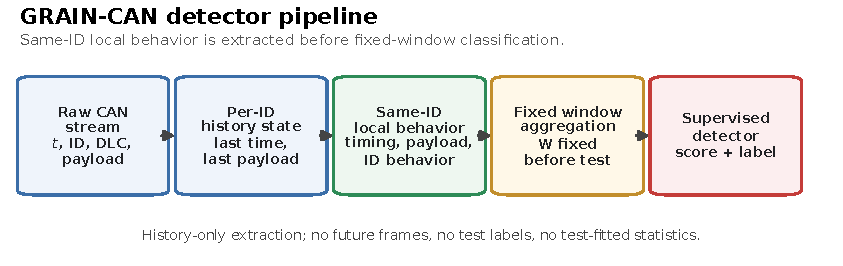
\includegraphics[width=\textwidth]{figures/fig1_grain_pipeline.pdf}
\caption{\method{} is a detector pipeline: it converts raw CAN frames into same-ID local behavior features before fixed-window supervised classification.}
\label{fig:pipeline}
\end{figure}

\begin{figure}[H]
\centering
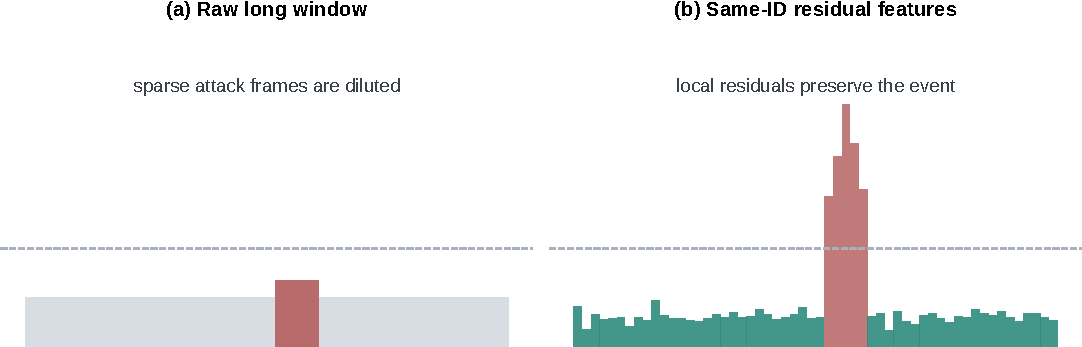
\includegraphics[width=\textwidth]{figures/fig2_local_evidence_mechanism.pdf}
\caption{Feature-before-window extraction keeps sparse local attack evidence visible before aggregation, whereas raw long windows can numerically dilute the same event.}
\label{fig:mechanism}
\end{figure}

\section{\method{} Pipeline}
\subsection{Overview}
\method{} has four stages: per-ID history maintenance, frame-level same-ID local behavior extraction, fixed pre-test window aggregation, and supervised classification. Unlike raw-window neural detectors that learn directly from a fixed sequence of frames, \method{} first converts each frame into local behavior residuals relative to the recent history of the same CAN ID.

\subsection{Input Stream and Per-ID History State}
The input stream is \(x_i=(t_i,id_i,dlc_i,b_i)\), where \(t_i\) is the timestamp, \(id_i\) is the arbitration ID, \(dlc_i\) is the data length, and \(b_i\) denotes the payload bytes. For every ID, \method{} maintains a compact state consisting of the last timestamp, last payload, recent counters, and recent summary statistics. The state is updated online and uses only current and past frames.

\subsection{Same-ID Local Behavior Feature Extraction}
The extracted features are grouped by purpose. Timing residuals capture disruptions in periodicity or burst patterns. Payload-change residuals capture discontinuities in byte-level behavior. Payload statistics summarize coarse byte distribution without requiring DBC decoding. Local ID-behavior features capture short concentration and frequency changes. These groups are later aggregated into fixed windows.

\subsection{Window Construction and Labeling}
Frame features are aggregated into fixed windows such as W10, W20, or W100. The window size is a configuration fixed before testing. A window is labelled attack if any frame in the window is labelled attack. This rule is common for window-level IDS experiments, but it also means rare attack windows can contain many normal frames; the design of \method{} is intended to keep the local evidence visible before the label is applied.

\subsection{Supervised Detector and Score Output}
In the repository experiments, \method{} uses a gradient-boosting tree ensemble. The classifier is not the main contribution; it learns a joint decision boundary over interpretable same-ID local behavior features. When the classifier exposes a score, we report AUPR and fixed-FPR detection rates as supplementary operating evidence.
\begin{table}[H]
\caption{Compared IDS pipelines. GRAIN-CAN differs in representation before aggregation rather than in classifier complexity.}\label{tab:pipelines}
\centering\small
\setlength{\tabcolsep}{3pt}
\begin{tabular}{>{\raggedright\arraybackslash}p{0.14\textwidth}>{\raggedright\arraybackslash}p{0.31\textwidth}>{\raggedright\arraybackslash}p{0.18\textwidth}>{\raggedright\arraybackslash}p{0.27\textwidth}}
\hline
Detector & Representation & Classifier & Purpose \\
\hline
Public GB & sample public-style features & GB & classical reproduced baseline \\
Public MLP & sample public-style features & MLP & neural classical baseline \\
Raw-Trans & raw fixed frame sequence, W100 & Transformer & raw-window deep baseline \\
GRAIN-W100 & same-ID local behavior features, W100 & GB & proposed detector pipeline \\
\hline
\end{tabular}
\end{table}

\subsection{Training and Inference Protocol}
\paragraph{Algorithm 1: training.}
Given a fixed window size \(W\), initialize an empty per-ID history table. Process the training stream in timestamp order. For each frame, read the current state of its CAN ID, compute local behavior features, update the state with the current frame, and append the feature vector to the current window. After every \(W\) frames, aggregate the frame features into a window vector and assign an attack label if any frame in the window is attack. Fit the supervised detector on training windows and, if a score threshold is required, select it on validation data.

\paragraph{Algorithm 1: inference.}
Freeze the feature definitions, window size, detector, and threshold. Process the test stream once in timestamp order. For each frame, compute features from current and past traffic only, update the per-ID state, aggregate windows, and emit a score or label. Test labels are used only after inference for evaluation.

\subsection{Relation to Existing Pipeline Types}
\method{} is not intended to replace signal-level, graph, self-supervised, or deep sequence IDS frameworks. Its scope is narrower: a lightweight supervised representation pipeline that exposes same-ID local behavior before aggregation and can be evaluated under cross-shift settings.
\begin{table}[H]
\caption{Positioning against representative CAN IDS pipeline families.}\label{tab:positioning}
\centering\small
\setlength{\tabcolsep}{3pt}
\begin{tabular}{>{\raggedright\arraybackslash}p{0.13\textwidth}>{\raggedright\arraybackslash}p{0.31\textwidth}>{\raggedright\arraybackslash}p{0.22\textwidth}>{\raggedright\arraybackslash}p{0.25\textwidth}}
\hline
Work & Core mechanism & Required information & Difference \\
\hline
CANShield & signal-level multi-scale autoencoder ensemble & DBC / signal extraction & GRAIN uses raw fields and no AE ensemble \\
X-CANIDS & signal-aware explainable detection & CAN database / signal semantics & GRAIN does not require decoded signals \\
CANet & message-level unsupervised neural detector & raw CAN messages & GRAIN is supervised and window-aggregated \\
MIDS & bidirectional Mamba sequence model & message sequence & GRAIN is a feature pipeline, not a deep backbone \\
GRAIN-CAN & same-ID local behavior before aggregation & timestamp, ID, DLC, payload & proposed lightweight supervised pipeline \\
\hline
\end{tabular}
\end{table}

\section{Related Work}
\subsection{Rule, Statistical, and Timing CAN IDS}
Early CAN IDS work often used message timing, ID frequency, and interval statistics because many injection attacks perturb periodic traffic. These approaches are attractive for deployment because they are lightweight and interpretable~\cite{song2016intrusion,taylor2016frequency,blevins2021time}. Their weakness is that a single statistic can miss attacks that preserve timing or shift behavior across vehicles. GRAIN-CAN keeps the lightweight spirit but uses multiple local residual features jointly through a supervised classifier.

\subsection{Deep Sequence and Representation Learning}
Deep CAN IDS methods learn from raw message sequences, payload bits, language-model-style tokenization, or modern sequence backbones~\cite{alkhatib2022canbert,liu2026mids}. These methods can learn rich dependencies but often require larger training sets, careful protocol design, and more compute. GRAIN-CAN takes a different route: it exposes local behavior changes with explicit features before any classifier sees a window.

\subsection{Signal-Level and Explainable Frameworks}
Signal-level frameworks such as CANShield and X-CANIDS use decoded signals or semantic signal structure to improve detection and interpretability~\cite{shahriar2022canshield,xcanids2023}. This is powerful when DBC or signal-level information is available. GRAIN-CAN uses only raw CAN fields and same-ID history, so it is easier to apply when signal definitions are unavailable.

\subsection{Unsupervised and Historical Models}
Unsupervised and historical models such as CANet learn normal message behavior without attack labels~\cite{canet2019}. GRAIN-CAN is supervised and should not be framed as solving arbitrary zero-day detection. Its value is narrower: it tests whether history-based local residuals improve cross-shift supervised detection when labels exist.

\section{Experimental Setup}
\subsection{Datasets and Cross-Shift Settings}
CT\&T set01 is the main dataset. Test01 uses a known vehicle and known attack families; Test02 changes the vehicle; Test03 changes the attack family; Test04 changes both. This gives a compact vehicle-shift and attack-shift matrix.
\begin{table}[H]
\caption{CT\&T cross-shift settings used in the main evaluation.}\label{tab:settings}
\centering\small
\resizebox{\textwidth}{!}{%
\begin{tabular}{lllrll}
\hline
Setting & Vehicle shift & Attack shift & Frames & Positive rate & Role \\
\hline
Test01 & known & known & 16355810 & 0.007 & known-vehicle known-attack baseline \\
Test02 & unknown & known & 17101057 & 0.012 & vehicle-shift stress test \\
Test03 & known & unknown & 19288415 & 0.004 & attack-shift stress test \\
Test04 & unknown & unknown & 23873695 & 0.003 & joint vehicle/attack-shift stress test \\
\hline
\end{tabular}
}
\end{table}

\subsection{Compared IDS Pipelines}
The main comparison keeps only representative detectors: public-style classical GradientBoosting and MLP rows, a raw fixed-window Transformer, and GRAIN-CAN windows. Simple single-signal thresholds are treated as diagnostic checks outside the main figure.

\subsection{Metrics and Threshold Rules}
Attack is the positive class. We report precision, recall, F1, FNR, and FPR from the confusion matrix. AUPR, AUROC, and recall at fixed FPR are supplementary because they require comparable scores. Window size and threshold must be fixed before test evaluation.

\subsection{Implementation Details}
The GRAIN rows use history-only features over timestamp, ID, DLC, payload bytes, same-ID timing residuals, payload-change residuals, payload statistics, and local ID behavior. W10, W20, and W100 are reported as configurations rather than test-selected winners.

\section{Evaluation}
\subsection{Cross-Shift Detection Results}
Table~\ref{tab:main} and Fig.~\ref{fig:main} summarize the main cross-shift results. The key pattern is not that one detector wins every setting. Rather, GRAIN-CAN provides strong attack-positive detection under vehicle and attack shifts, especially compared with raw fixed-window behavior in Test02 and Test04.
\begin{table}[H]
\caption{Main CT\&T results with attack as the positive class.}\label{tab:main}
\centering\small
\begin{tabular}{lllllll}
\hline
Setting & Detector & P & R & F1 & FNR & FPR \\
\hline
Test01 & GB-sample & 0.860 & 0.980 & 0.916 & 0.020 & 0.001 \\
Test01 & MLP & 0.209 & 0.365 & 0.266 & 0.635 & 0.010 \\
Test01 & Raw-Trans & 1.000 & 0.931 & 0.964 & 0.069 & 0.000 \\
Test01 & GRAIN-W100 & 0.999 & 0.892 & 0.942 & 0.108 & 0.000 \\
Test02 & GB-sample & 0.931 & 0.998 & 0.964 & 0.002 & 0.001 \\
Test02 & MLP & 0.283 & 0.933 & 0.434 & 0.067 & 0.030 \\
Test02 & Raw-Trans & 0.087 & 1.000 & 0.160 & 0.000 & 0.133 \\
Test02 & GRAIN-W100 & 0.984 & 0.931 & 0.956 & 0.069 & 0.000 \\
Test03 & GB-sample & 0.719 & 0.629 & 0.671 & 0.371 & 0.001 \\
Test03 & MLP & 0.087 & 0.574 & 0.151 & 0.426 & 0.022 \\
Test03 & Raw-Trans & 1.000 & 0.013 & 0.025 & 0.987 & 0.000 \\
Test03 & GRAIN-W100 & 1.000 & 0.662 & 0.797 & 0.338 & 0.000 \\
Test04 & GB-sample & 0.707 & 0.447 & 0.548 & 0.553 & 0.000 \\
Test04 & MLP & 0.002 & 0.077 & 0.004 & 0.923 & 0.089 \\
Test04 & Raw-Trans & 0.011 & 0.980 & 0.022 & 0.020 & 0.229 \\
Test04 & GRAIN-W100 & 0.938 & 0.519 & 0.668 & 0.481 & 0.000 \\
\hline
\end{tabular}
\end{table}

\begin{figure}[H]
\centering
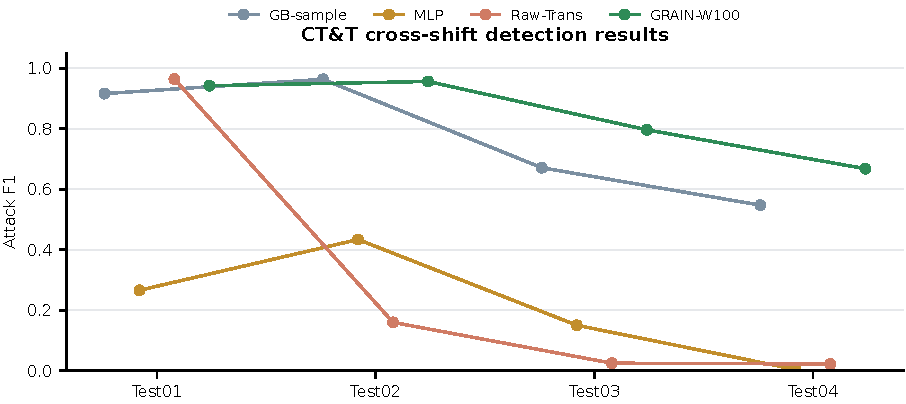
\includegraphics[width=\textwidth]{figures/fig3_main_ctt_results.pdf}
\caption{GRAIN-CAN remains competitive across CT\&T shifts, while the raw fixed-window Transformer collapses in vehicle-shifted settings.}
\label{fig:main}
\end{figure}

\subsection{Effect of Feature-Before-Window Representation}
The raw-window comparison isolates the representation effect. Both pipelines use fixed windows, but only GRAIN-CAN extracts same-ID local behavior before aggregation. The contrast is strongest in Test02 and Test04, where raw windows produce high miss or false-alarm behavior.
\begin{table}[H]
\caption{Raw fixed-window pipeline versus GRAIN-CAN.}\label{tab:rawgrain}
\centering\small
\begin{tabular}{llllll}
\hline
Setting & Pipeline & P & R & F1 & AUPR \\
\hline
Test01 & GRAIN-W100 & 0.999 & 0.892 & 0.942 & 0.896 \\
Test01 & Raw-Trans & 1.000 & 0.931 & 0.964 & 0.984 \\
Test02 & GRAIN-W100 & 0.984 & 0.931 & 0.956 & 0.935 \\
Test02 & Raw-Trans & 0.087 & 1.000 & 0.160 & 0.049 \\
Test03 & GRAIN-W100 & 1.000 & 0.662 & 0.797 & 0.925 \\
Test03 & Raw-Trans & 1.000 & 0.013 & 0.026 & 0.271 \\
Test04 & GRAIN-W100 & 0.936 & 0.519 & 0.668 & 0.785 \\
Test04 & Raw-Trans & 0.011 & 0.979 & 0.022 & 0.173 \\
\hline
\end{tabular}
\end{table}

\begin{figure}[H]
\centering

\includegraphics[width=\textwidth]{figures/fig4_raw_vs_grain.pdf}
\caption{The same W100 aggregation becomes more reliable when local behavior residuals are computed before the window is formed.}
\label{fig:rawgrain}
\end{figure}

\subsection{Contribution of Local Behavior Features}
Feature-group ablation on Test04 shows that same-ID timing is the strongest individual signal in the current setting. Removing same-ID timing sharply degrades F1, while payload and ID groups have weaker effects. This supports the pipeline's focus on residual behavior rather than absolute payload values alone.
\begin{table}[H]
\caption{Feature-group ablation on CT\&T Test04.}\label{tab:ablation}
\centering\small
\begin{tabular}{llllllll}
\hline
Variant & P & R & F1 & FNR & FPR & AUPR & R@1e-3 \\
\hline
Timing only & 0.771 & 0.491 & 0.600 & 0.509 & 0.000 & 0.425 & 0.491 \\
w/o CAN ID & 0.740 & 0.355 & 0.480 & 0.645 & 0.000 & 0.265 & 0.355 \\
Full safe features & 0.740 & 0.354 & 0.479 & 0.646 & 0.000 & 0.255 & 0.355 \\
w/o payload stats & 0.740 & 0.354 & 0.479 & 0.646 & 0.000 & 0.255 & 0.355 \\
w/o payload delta & 0.740 & 0.354 & 0.479 & 0.646 & 0.000 & 0.255 & 0.355 \\
w/o same-ID timing & 0.005 & 0.249 & 0.009 & 0.751 & 0.056 & 0.057 & 0.067 \\
\hline
\end{tabular}
\end{table}

\begin{figure}[H]
\centering
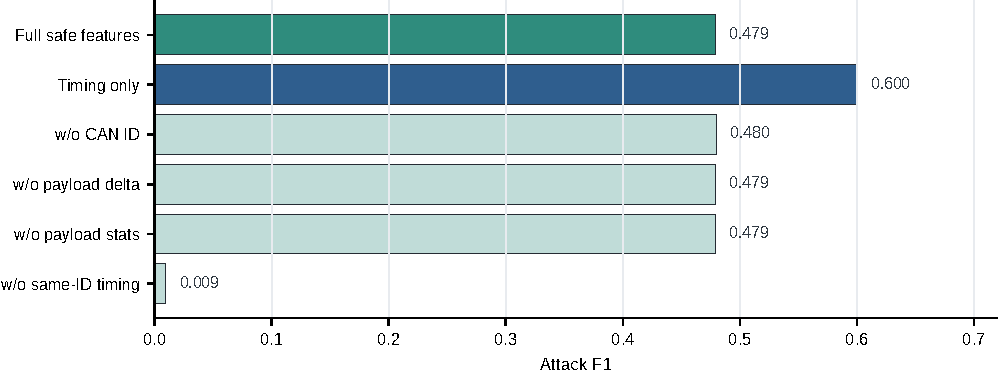
\includegraphics[width=\textwidth]{figures/fig5_feature_ablation.pdf}
\caption{Ablation identifies same-ID timing residuals as the strongest local behavior signal in Test04.}
\label{fig:ablation}
\end{figure}

\subsection{Sensitivity to Aggregation Window}
W10, W20, and W100 behave differently across settings. Shorter windows help Test01 and Test02, while W100 is stronger in Test03 and Test04. The result argues for reporting window sensitivity instead of treating one test-selected window as a universal hyperparameter.

\subsection{Low-False-Alarm Operating Points}
Score-based operating analysis is supplementary. Fig.~\ref{fig:opfpr} compares AUPR and the available fixed-FPR detection evidence on Test04. These metrics are useful for deployment discussions, but they are reported only when the underlying score is available under the same protocol.
\begin{figure}[H]
\centering
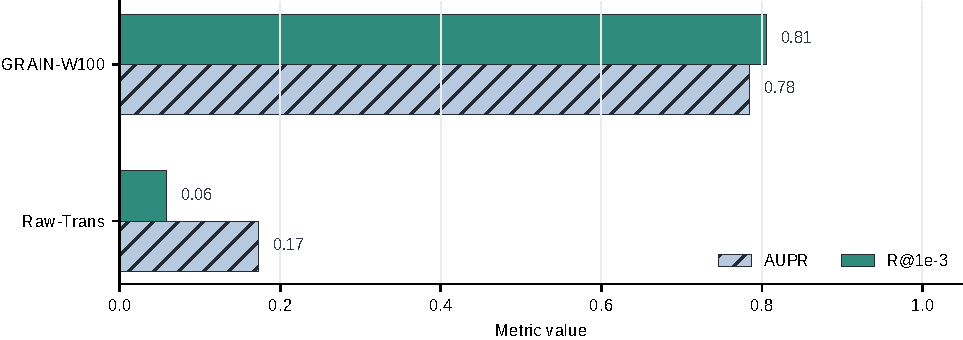
\includegraphics[width=\textwidth]{figures/fig6_low_fpr_operating.pdf}
\caption{Supplementary Test04 operating evidence shows that AUPR and fixed-FPR recall must be interpreted separately from thresholded F1.}
\label{fig:opfpr}
\end{figure}

\subsection{Diagnostic Rule and Statistical Checks}
We include simple single-signal detectors only as diagnostic checks. They test whether GRAIN-CAN is merely a single threshold over timing or payload change. They are not presented as recent state-of-the-art competitors.

\section{Discussion}
\subsection{What GRAIN-CAN Explains}
The experiments support the design claim that local same-ID behavior should be made explicit before window aggregation. GRAIN-CAN is strongest when raw windows struggle to preserve sparse evidence under vehicle or attack shifts.

\subsection{Failure Modes}
\method{} still needs supervised labels and visible disruptions in timing, payload continuity, or local ID behavior. Attacks that preserve those properties can be missed. The method is also not vehicle-independent: it reduces reliance on absolute distributions but does not remove distribution shift.

\subsection{Comparability to Prior Work}
Prior reported aggregate metrics cannot be directly compared with attack-positive F1 unless the positive class, averaging rule, thresholds, and confusion matrix are available. We therefore compare reproduced local rows under a common metric definition and treat score metrics as supplementary.

\section{Conclusion}
\method{} demonstrates that same-ID local behavior extraction before window aggregation is a useful lightweight design for cross-shift CAN IDS. Its strength is interpretable representation-level robustness; its limitation is that supervised labels and visible timing or payload disruptions are still required. Future work should combine this representation with self-supervised training, signal-level features, DBC-aware variants, online adaptation, and real-time deployment evaluation.

\bibliographystyle{splncs04}
\bibliography{grain_can_framework_refs}
\end{document}
